% !TeX program = pdfLaTeX
\documentclass[12pt]{article}
\usepackage{amsmath}
\usepackage{amsthm}
\usepackage{graphicx,psfrag,epsf}
\usepackage{enumerate}
\usepackage{natbib}
\usepackage{booktabs}
\usepackage{longtable}
\usepackage{array}
\usepackage{adjustbox}
\usepackage{multirow}
\usepackage{subfig}
\usepackage[table]{xcolor}
\usepackage{wrapfig}
\usepackage{float}
\usepackage{colortbl}
\usepackage{hyperref}
\usepackage{pdflscape}
\usepackage{tabu}
\usepackage{threeparttable}

\usepackage{url} % not crucial - just used below for the URL

%\pdfminorversion=4
% NOTE: To produce blinded version, replace "0" with "1" below.
\newcommand{\blind}{0}

% DON'T change margins - should be 1 inch all around.
\addtolength{\oddsidemargin}{-.5in}%
\addtolength{\evensidemargin}{-.5in}%
\addtolength{\textwidth}{1in}%
\addtolength{\textheight}{1.3in}%
\addtolength{\topmargin}{-.8in}%

\newenvironment{definition}[1]% environment name 
{% begin code 
  \par\vspace{.75\baselineskip}\noindent 
  \textbf{Definition (#1)}\begin{itshape}% 
  \par\vspace{.5\baselineskip}\noindent\ignorespaces 
}% 
{% end code 
  \end{itshape}\ignorespacesafterend 
}

\providecommand{\tightlist}{%
  \setlength{\itemsep}{0pt}\setlength{\parskip}{0pt}}

\begin{document}

\def\spacingset#1{\renewcommand{\baselinestretch}%
{#1}\small\normalsize} \spacingset{1}


%%%%%%%%%%%%%%%%%%%%%%%%%%%%%%%%%%%%%%%%%%%%%%%%%%%%%%%%%%%%%%%%%%%%%%%%%%%%%%


  % \bigskip

  % \bigskip
\newpage

\if0\blind
{
  \title{\LARGE\bf APPENDIX \\ Adapting the Chumbley Score to match striae on Land Engraved Areas (LEAs) of bullets}
  \maketitle
} \fi

% \if1\blind
% {
%   \bigskip
%   \bigskip
%   \bigskip
%   \begin{center}
%     {\LARGE\bf Adapting the Chumbley Score to match striae on Land Engraved Areas}
%   \end{center}
%   \medskip
% } \fi
%
%\bigskip
%\begin{abstract}
%The same-source problem remains a major challenge in forensic toolmark
%and firearm examination. Technological advances in surface imaging allow
%measurements of 3D surfaces at previously unforeseen resolutions and
%enable digitized imaging. Here, we investigate the applicability of the
%Chumbley scoring method \citep{hadler}, developed for screwdriver
%markings, for same-source identification of bullet striae. We provide
%methods to identify parameters that minimize the error rates for
%matching of LEAs using Hamby datasets 44 and 252 measured by NIST and
%CSAFE. We suggest a remedial algorithm to alleviate the problem of
%failed tests in the method, increasing both the power of the test and
%reducing error rates. Type II error rates of the proposed method improve
%by more than one third (Type I error of 0.05) and are on average about
%0.22. This puts the proposed method on similar footing as other single
%feature matching approaches in the literature.
%\end{abstract}
%
%\noindent%
%{\it Keywords:} forensic science, toolmark, cross-correlation, Mann-Whitney U statistic, land engraved areas (LEAs), algorithm, signatures, same-source problem
%\vfill

\newpage
\spacingset{1.45} % DON'T change the spacing!

\newcommand{\cited}[1]{{\textcolor{red}{#1}}}

\setlength\parindent{0pt}

%\tableofcontents
%\newpage
\section*{Appendix}\label{appendix}

\begin{appendix}

\section{Scenarios of failed tests}
\label{appendix:appxfailed}
Figures \ref{same-shift-failure} and \ref{diff-shift-failure} show scenarios in which the deterministic Chumbley score can fail. 
In \autoref{same-shift-failure} both CS1 and CS2 fail, because the lag between optimal locations is so large that no same-shift pairs can be found once the signatures are aligned. These failures are inherent to the Chumbley Score and cannot be prevented.
\begin{figure}[hbtp]
\centering
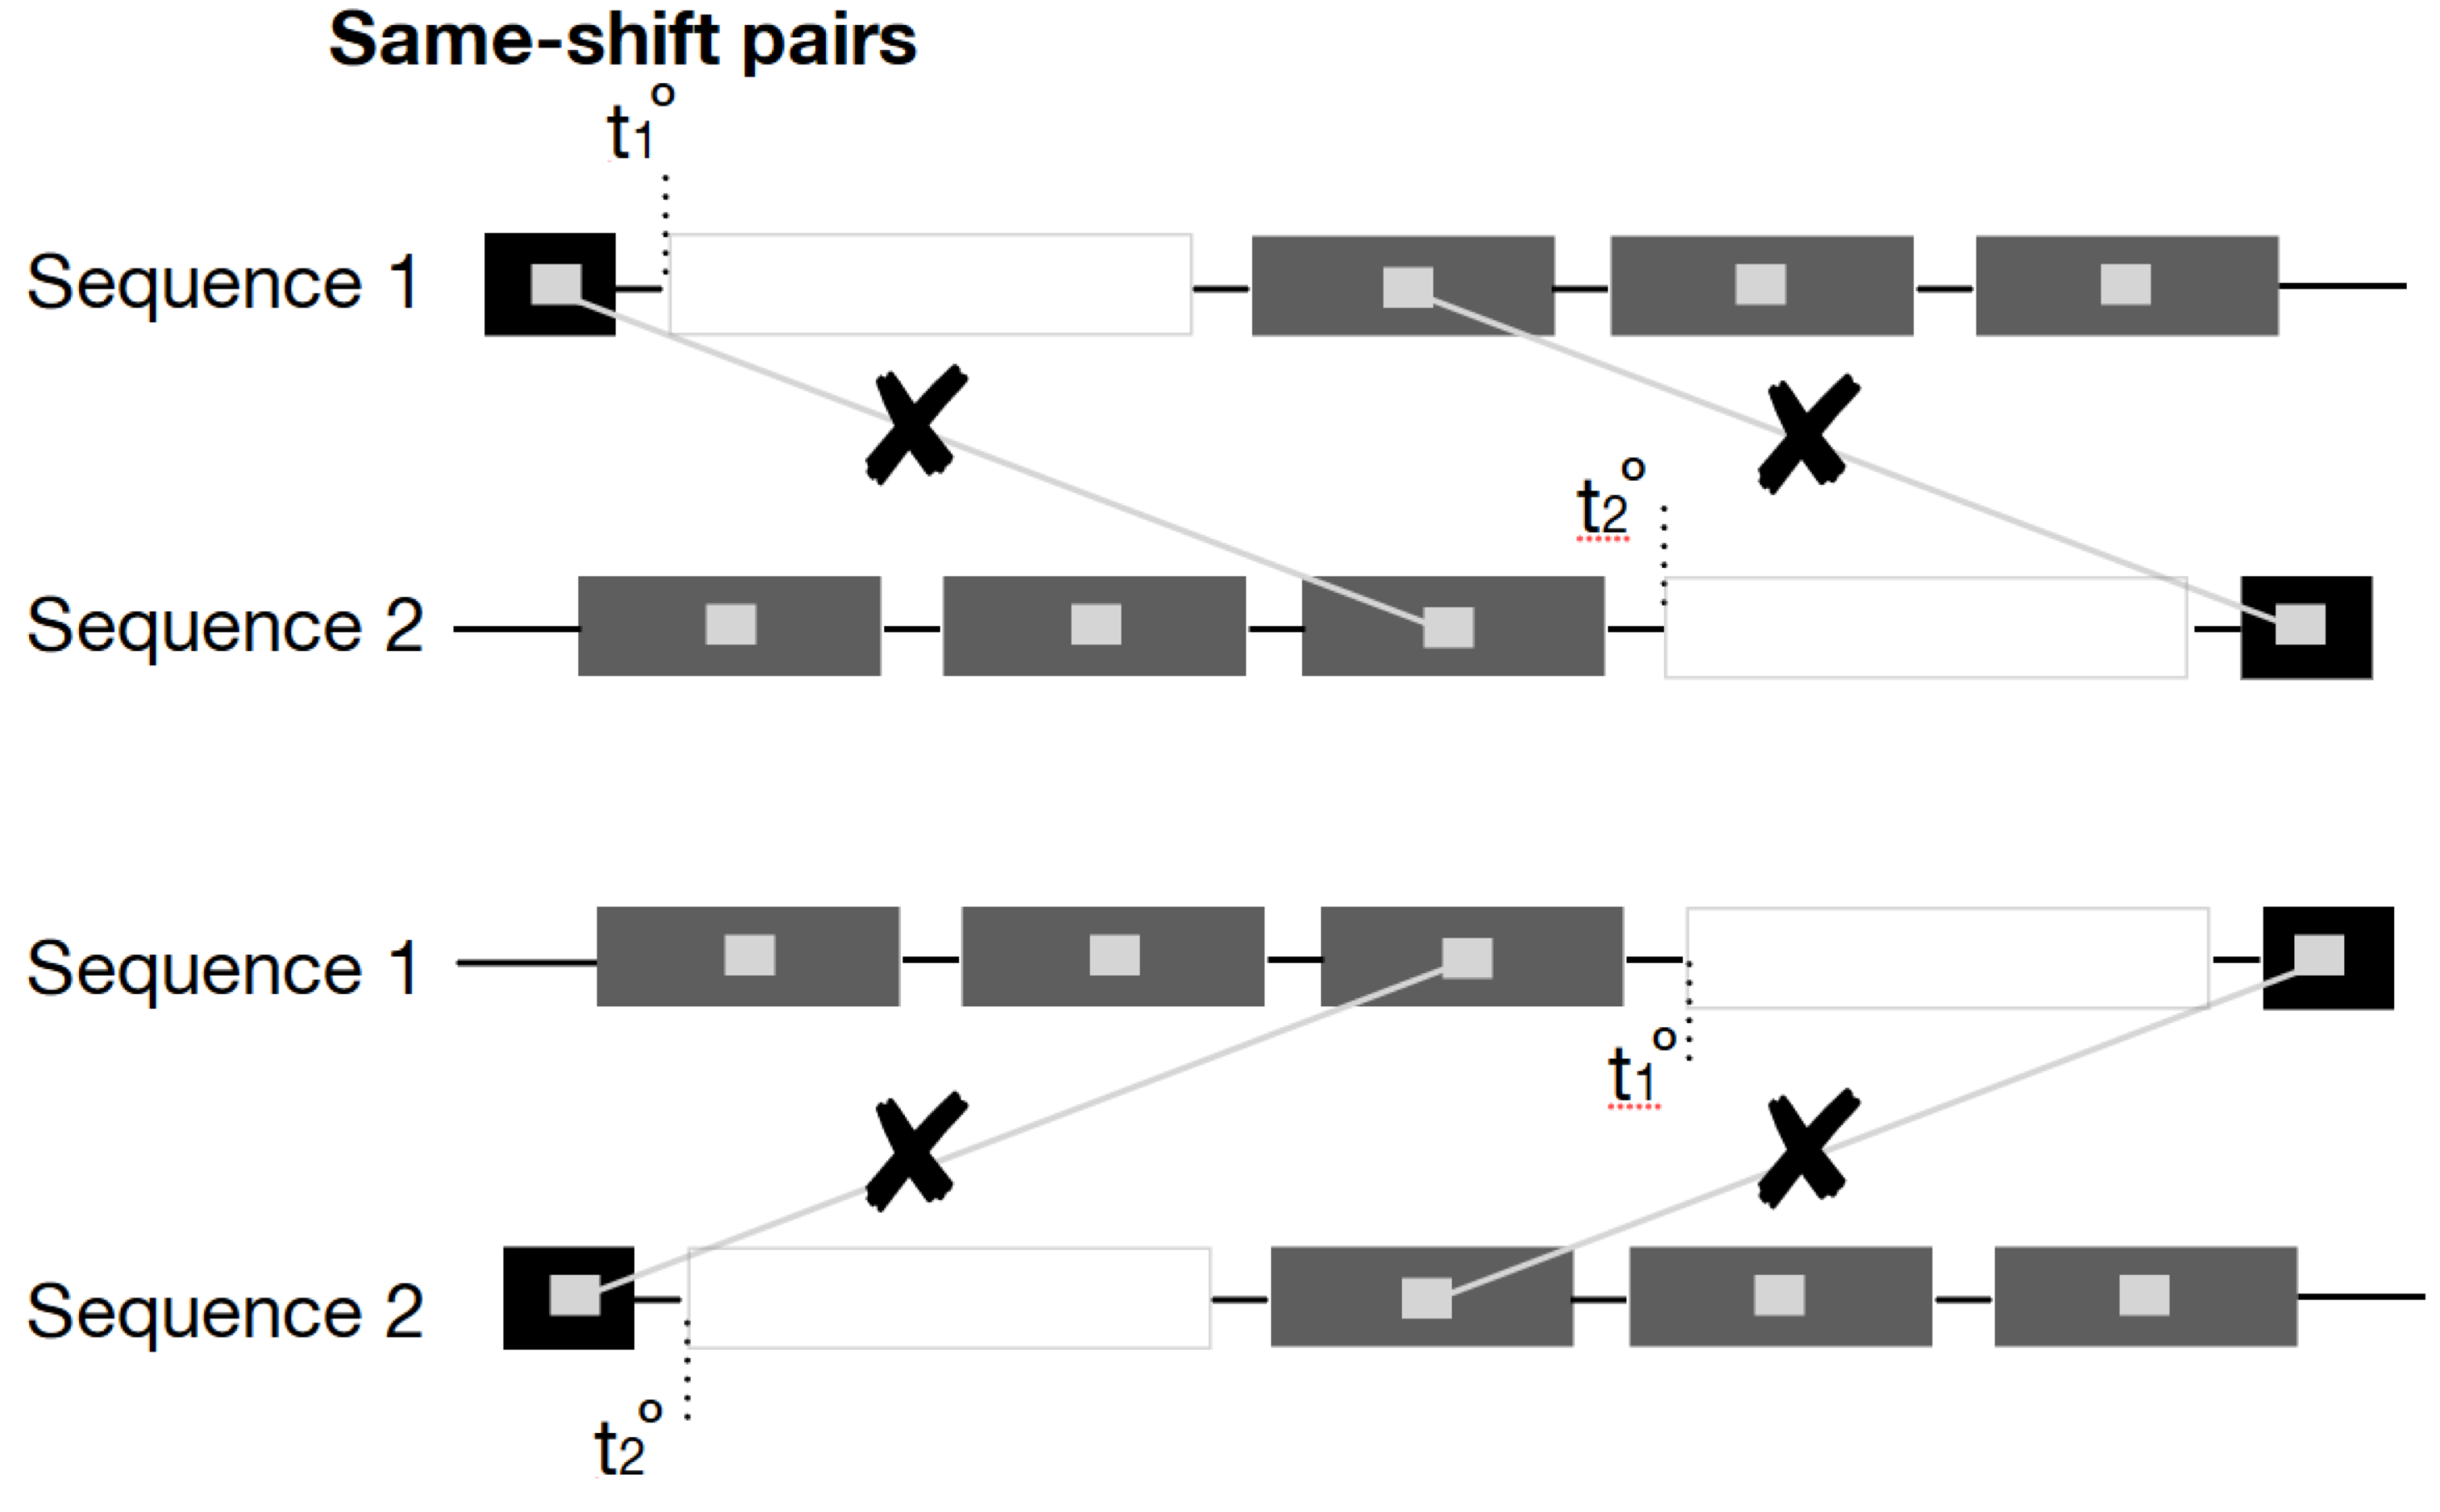
\includegraphics[width=0.62\textwidth]{images/same-shift-failure.png}

\caption{\label{same-shift-failure}Sketch of same-shift pairings. When the lag between optimal reference points is too large to accommodate a validation window in both signatures, both CS1 and CS2 fail.}
\end{figure}

\autoref{diff-shift-failure} shows two situations, in which CS1 fails to identify any different-shift pairings. This happens, when both relative locations are close to either end of the signature. CS2 can still be computed in this situation as long as there are at least two same-shift pairs identified. 

\begin{figure}[hbtp]
\centering
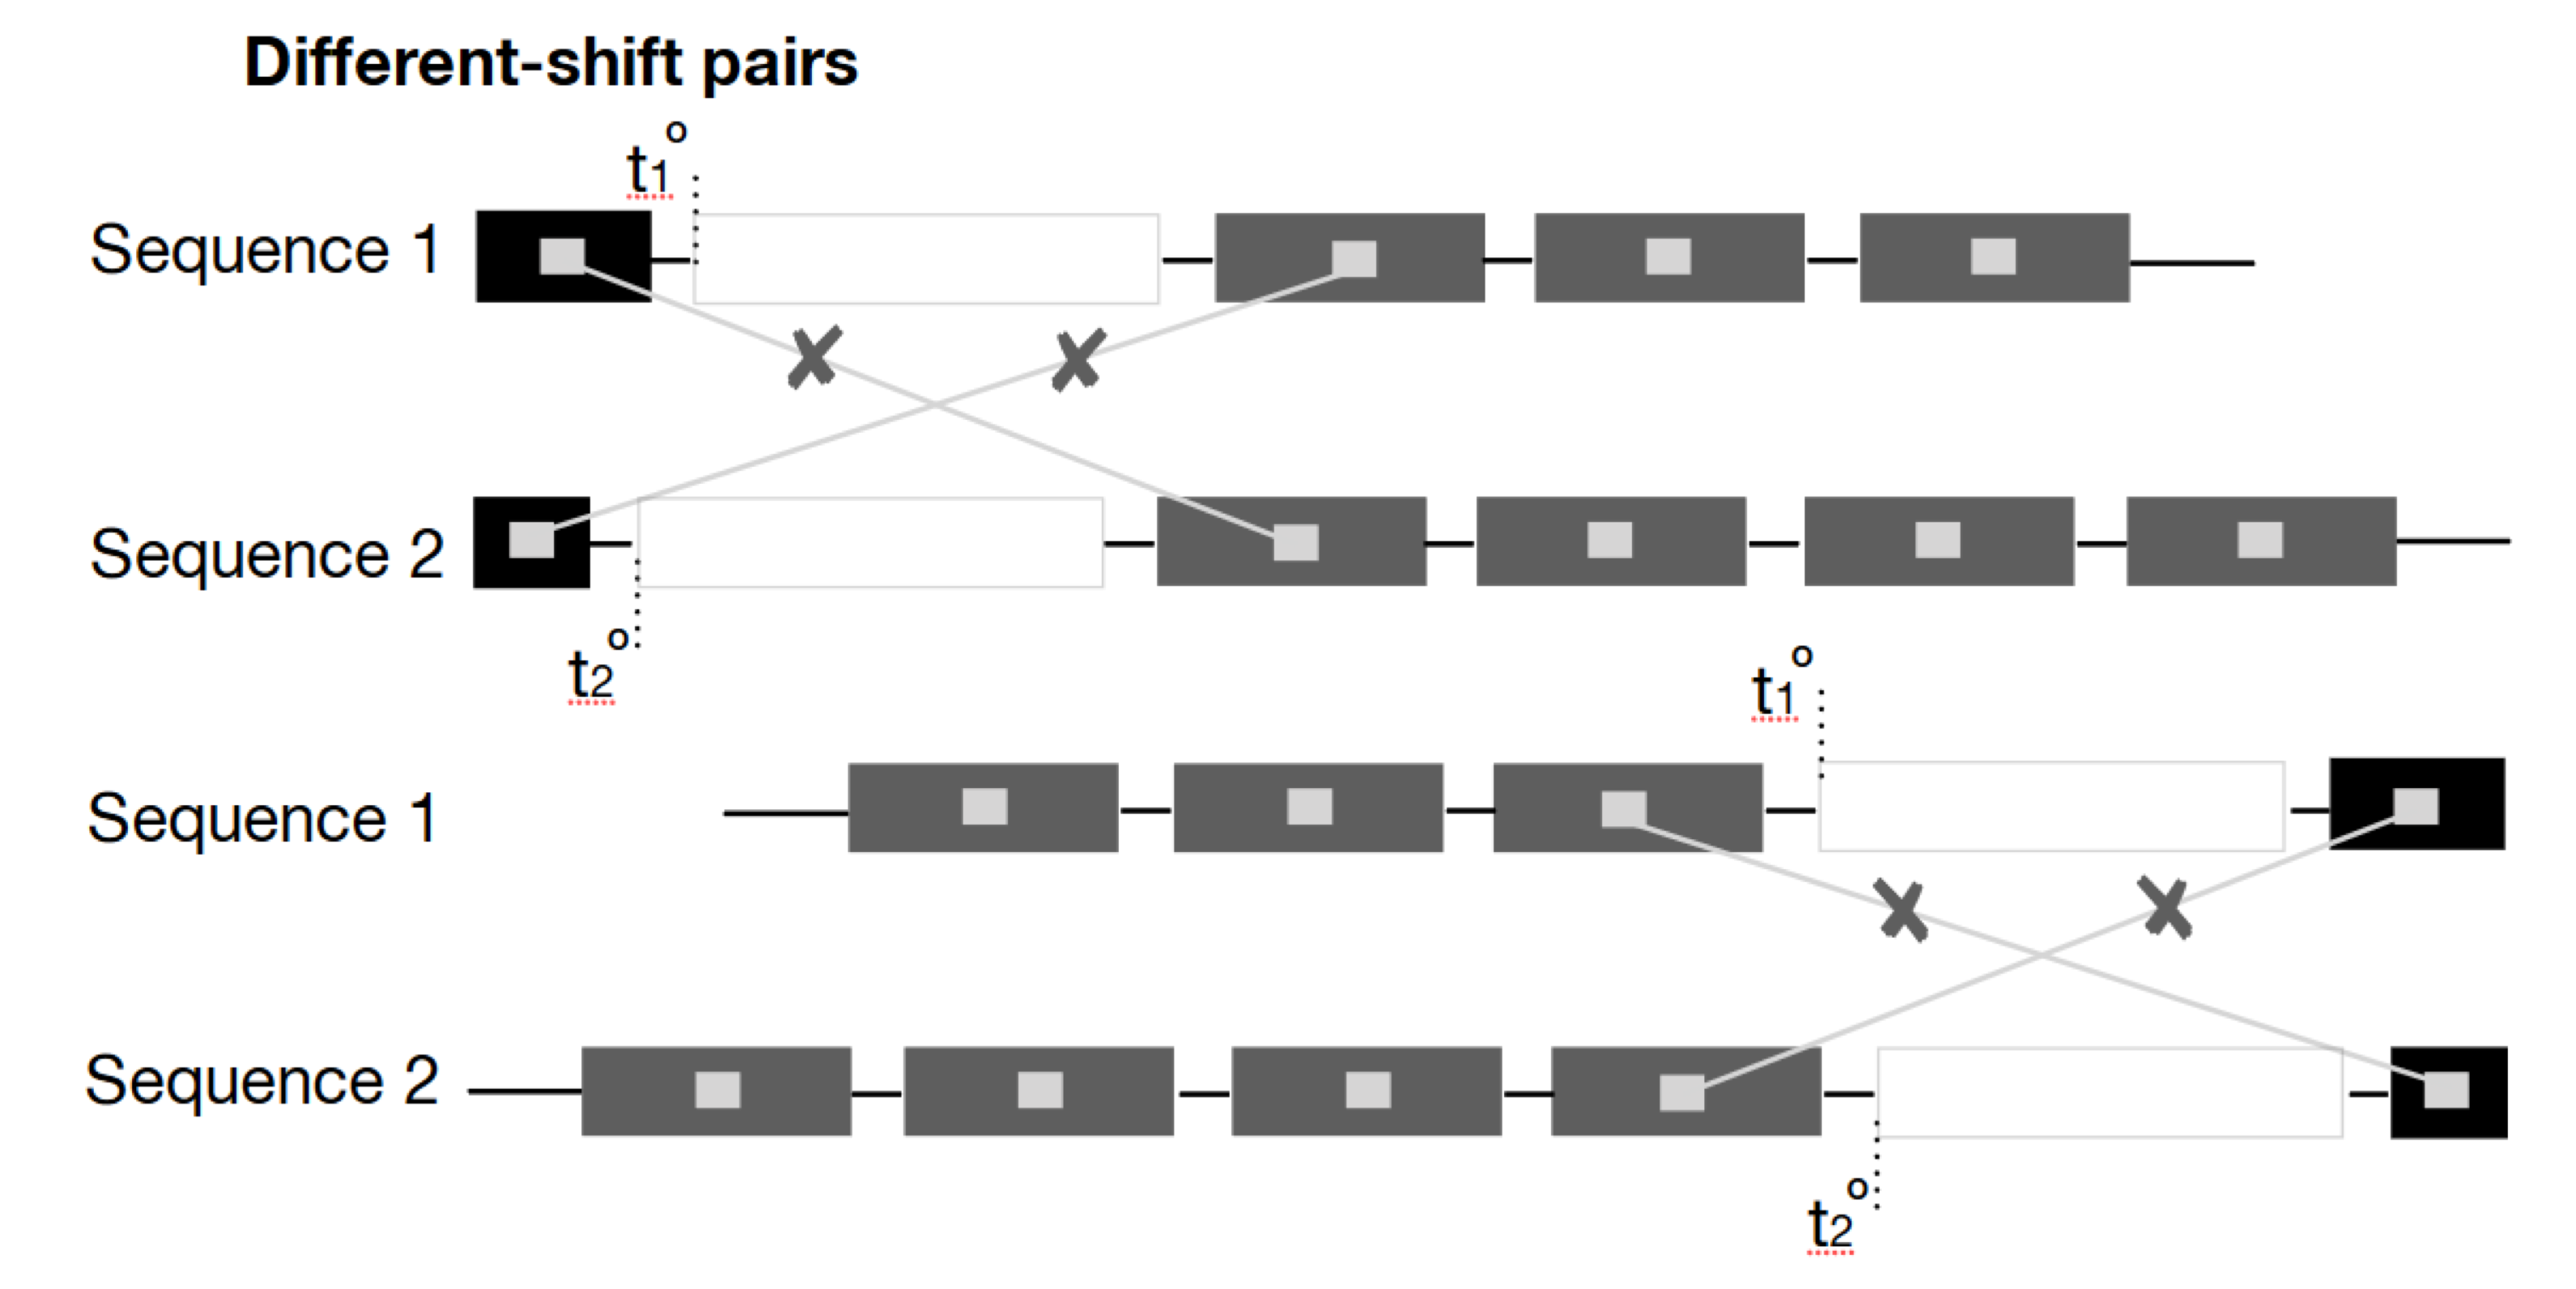
\includegraphics[width=0.7\textwidth]{images/diff-shift-failure.png}

\caption{\label{diff-shift-failure}Sketch of different-shift pairings. For CS1 no different-shift pairs can be identified, resulting in a failed test.}
\end{figure}

\newpage
\section{Type 2 errors: CS1 vs CS2}
\label{appendix:appxtype2}
\autoref{fig:type2} gives an overview of type 2 error rates of methods CS1 and CS2 for different significance levels $\alpha$. Method CS2 is outperforming CS1 significantly in every instance.

\begin{figure}[h]

{\centering 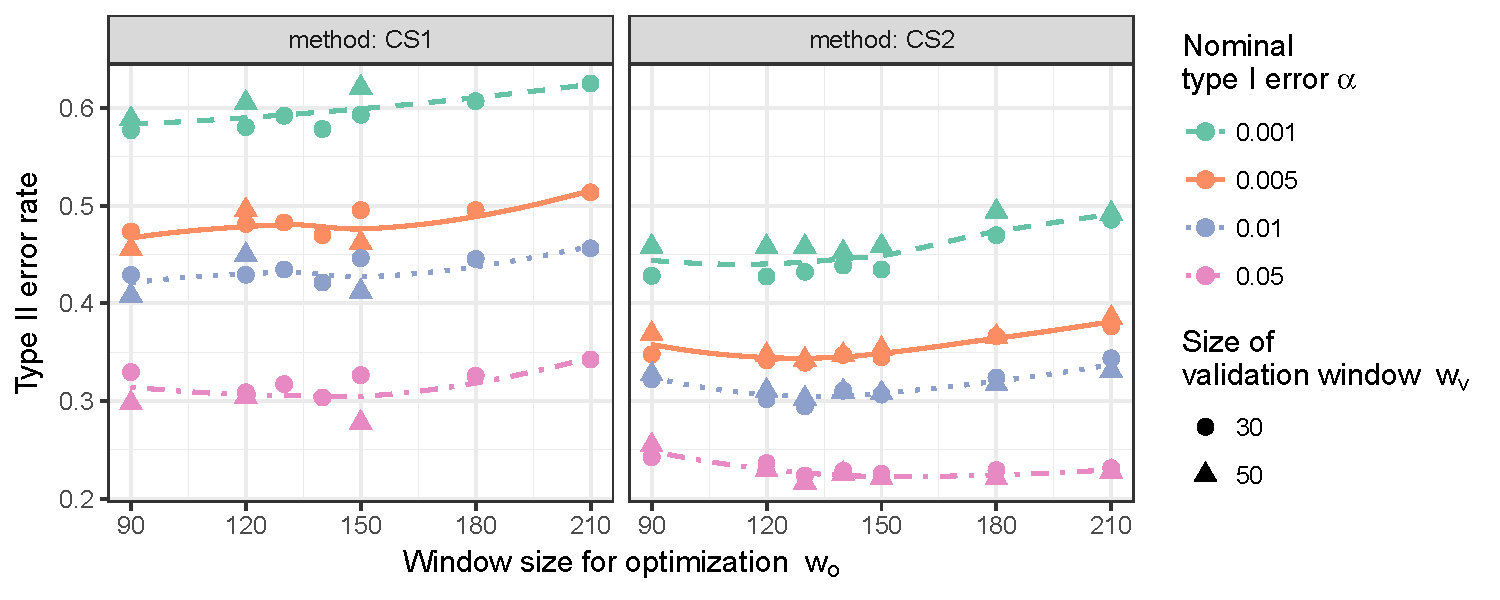
\includegraphics[width=0.9\textwidth]{figures/type2-1} 

}

\caption{Type II error rates observed across a range of window sizes for optimization $w_o$. For a window size of $w_o = 130$ we see a minimum in type II error rate across all type I rates considered. Smaller validation sizes $w_v$ are typically associated with a smaller type II error.}\label{fig:type2}
\end{figure}

\end{appendix}

%\bibliographystyle{agsm}
%\bibliography{bibliography}

\end{document}
